\chapter{MOA Experimental Setting}
\label{chap:experimentalsetting} 

This chapter establishes the settings under which stream mining experiments may be conducted, presenting the framework \textbf{MOA} %necessary
 to place various learning algorithms under test.
This experimental methodology %adopted by this \thesis 
is motivated by the requirements of the end user and their desired application.

\begin{figure}[ht]
\begin{center}
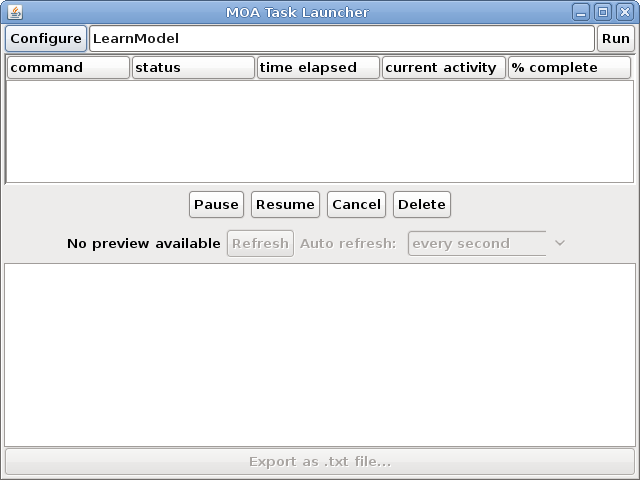
\includegraphics[height=6cm]{figures/MOATask.png}\end{center}
\caption{Graphical user interface of MOA}
\end{figure}

A user wanting to classify examples in a stream of data will have a set of requirements. They will have a certain volume of data, composed of a number of features per example, and a rate at which examples arrive. They will have the computing hardware on which the training of the model and the classification of new examples is to occur.
Users will naturally seek the most accurate predictions possible on the hardware provided. They are, however, more likely to accept a solution that sacrifices accuracy in order to function, than no solution at all. Within reason the user's requirements may be relaxed, such as reducing the training features or upgrading the hardware, but there comes a point at which doing so would be unsatisfactory.

The behaviour of a data stream learning algorithm has three dimensions of interest---the amount of space (computer memory) required, the time required to learn from training examples and to predict labels for new examples, and the error of the predictions.
When the user's requirements cannot be relaxed any further, the last remaining element that can be tuned to meet the demands of the problem is the {\em effectiveness} of the learning algorithm---the ability of the algorithm to output minimum error in limited time and space.

The error of an algorithm is the dimension that people would like to control the most, but it is the least controllable. The biggest factors influencing error are the {\em representational power} of the algorithm, how capable the model is at capturing the true underlying concept in the stream, and its {\em generalization power}, how successfully it can ignore noise and isolate useful patterns in the data.

Adjusting the time and space used by an algorithm can influence error. Time and space are interdependent. By storing more pre-computed information, such as look up tables, an algorithm can run faster at the expense of space. An algorithm can also run faster by processing less information, either by stopping early or storing less, thus having less data to process. The more time an algorithm has to process, or the more information that is processed, the more likely it is that error can be reduced.

The time and space requirements of an algorithm can be controlled by design. The algorithm can be optimised to reduce memory footprint and runtime. More directly, an algorithm can be made aware of the resources it is using and dynamically adjust. For example, an algorithm can take a memory limit as a parameter, and take steps to obey the limit. Similarly, it could be made aware of the time it is taking, and scale computation back to reach a time goal.

The easy way to limit either time or space is to stop once the limit is reached, and resort to the best available output at that point. For a time limit, continuing to process will require the user to wait longer, a compromise that may be acceptable in some situations. For a space limit, the only way to continue processing is to have the algorithm specifically designed to discard some of its information, hopefully information that is least important.
Additionally, time is highly dependent on physical processor implementation, whereas memory limits are universal.
The space requirement is a hard overriding limit that is ultimately dictated by the hardware available. An algorithm that requests more memory than is available will cease to function, a consequence that is much more serious than either taking longer, or losing accuracy, or both.

It follows that the space dimension should be fixed in order to evaluate algorithmic performance. 
Accordingly, to evaluate the ability of an algorithm to meet user requirements, a memory limit is set, and the resulting time and error performance of the algorithm is measured on a data stream.
Different memory limits have been chosen to gain insight into general performance of algorithmic variations by covering a range of plausible situations.

Several elements are covered in order to establish the evaluation framework used in this \thesisc. Evaluation methods already established in the field are surveyed in Section~\ref{sec:preveval}. Possible procedures are compared in~\ref{sec:evalcomp} and the final evaluation framework is described in Section~\ref{sec:framework}. The memory limits used for testing are motivated in Section~\ref{sec:environments}, and Section~\ref{sec:datasets} describes the data streams used for testing. Finally, Section~\ref{sec:genspeed} analyzes the speeds and sizes of the data streams involved. The particular algorithms under examination are the focus of the remainder of the \thesisc. 

\section{Previous Evaluation Practices}
\label{sec:preveval}

This section assumes that the critical variable being measured by evaluation processes is the {\em accuracy} of a learning algorithm. Accuracy, or equivalently its converse, {\em error}, may not be the only concern, but it is usually the most pertinent one. Accuracy is typically measured as the percentage of correct classifications that a model makes on a given set of data, the most accurate learning algorithm is the one that makes the fewest mistakes when predicting labels of examples. With classification problems, achieving the highest possible accuracy is the most immediate and obvious goal.
Having a reliable estimate of accuracy enables comparison of different methods, so that the best available method for a given problem can be determined.

It is very {\em optimistic} to measure the accuracy achievable by a learner on the same data that was used to train it, because even if a model achieves perfect accuracy on its training data this may not reflect the accuracy that can be expected on unseen data---its {\em generalization} accuracy.
For the evaluation of a learning algorithm to measure practical usefulness, the algorithm's ability to generalize to previously unseen examples must be tested. A model is said to {\em overfit} the data if it tries too hard to explain the training data, which is typically noisy, so performs poorly when predicting the class label of examples it has not seen before. One of the greatest challenges of machine learning is finding algorithms that can avoid the problem of overfitting.

\subsection{Batch Setting}

Previous work on the problem of evaluating batch learning has concentrated on making the best use of a limited supply of data.
When the number of examples available to describe a problem is in the order of hundreds or even less then reasons for this concern are obvious. When data is scarce, ideally all data that is available should be used to train the model, but this will leave no remaining examples for testing. The following methods discussed are those that have in the past been considered most suitable for evaluating batch machine learning algorithms, and are studied in more detail by Kohavi~\cite{cvstudy}.

% holdout

The {\em holdout} method divides the available data into two subsets that are mutually exclusive. One of the sets is used for training, the {\em training} set, and the remaining examples are used for testing, the {\em test} or {\em holdout} set. Keeping these sets separate ensures that generalization performance is being measured. Common size ratios of the two sets used in practice are 1/2 training and 1/2 test, or 2/3 training and 1/3 test. Because the learner is not provided the full amount of data for training, assuming that it will improve given more data, the performance estimate will be pessimistic. The main criticism of the holdout method in the batch setting is that the data is not used efficiently, as many examples may never be used to train the algorithm. The accuracy estimated from a single holdout can vary greatly depending on how the sets are divided. To mitigate this effect, the process of {\em random subsampling} will perform multiple runs of the holdout procedure, each with a different random division of the data, and average the results. Doing so also enables measurement of the accuracy estimate's variance. Unfortunately this procedure violates the assumption that the training and test set are independent---classes over-represented in one set will be under-represented in the other, which can skew the results. 

% cross-validation

In contrast to the holdout method, {\em cross-validation} maximizes the use of examples for both training and testing. In $k$-fold cross-validation the data is randomly divided into $k$ independent and approximately equal-sized {\em folds}. The evaluation process repeats $k$ times, each time a different fold acts as the holdout set while the remaining folds are combined and used for training. The final accuracy estimate is obtained by dividing the total number of correct classifications by the total number of examples. In this procedure each available example is used $k-1$ times for training and exactly once for testing. This method is still susceptible to imbalanced class distribution between folds. Attempting to reduce this problem, {\em stratified cross-validation} distributes the labels evenly across the folds to approximately reflect the label distribution of the entire data. Repeated cross-validation repeats the cross-validation procedure several times, each with a different random partitioning of the folds, allowing the variance of the accuracy estimate to be measured.

% leave-one-out

The {\em leave-one-out} evaluation procedure is a special case of cross-validation where every fold contains a single example. This means with a data set of $n$ examples that $n$-fold cross validation is performed, such that $n$ models are induced, each of which is tested on the single example that was held out. In special situations where learners can quickly be made to `forget' a single training example this process can be performed efficiently, otherwise in most cases this procedure is expensive to perform. The leave-one-out procedure is attractive because it is completely deterministic and not subject to random effects in dividing folds. However, stratification is not possible and it is easy to construct examples where leave-one-out fails in its intended task of measuring generalization accuracy. Consider what happens when evaluating using completely random data with two classes and an equal number of examples per class---the best an algorithm can do is predict the majority class, which will always be incorrect on the example held out, resulting in an accuracy of 0\%, even though the expected estimate should be 50\%.

% stratification

% bootstrap

An alternative evaluation method is the {\em bootstrap} method introduced by Efron~\cite{bootstrap}. This method creates a {\em bootstrap sample} of a data set by sampling with replacement a training data set of the same size as the original. Under the process of sampling with replacement the probability that a particular example will be chosen is approximately 0.632, so the method is commonly known as the 0.632 bootstrap. All examples not present in the training set are used for testing, which will contain on average about 36.8\% of the examples. The method compensates for lack of unique training examples by combining accuracies measured on both training and test data to reach a final estimate:
\begin{equation} \label{eq:bstrap}
accuracy_{bootstrap} = 0.632 \times accuracy_{test} + 0.368 \times accuracy_{train}
\end{equation}
As with the other methods, repeated random runs can be averaged to increase the reliability of the estimate. This method works well for very small data sets but suffers from problems that can be illustrated by the same situation that causes problems with leave-one-out, a completely random two-class data set---Kohavi~\cite{cvstudy} argues that although the true accuracy of any model can only be 50\%, a classifier that memorizes the training data can achieve $accuracy_{train}$ of 100\%, resulting in $accuracy_{bootstrap} = 0.632 \times 50\% + 0.368 \times 100\% = 68.4\%$. This estimate is more optimistic than the expected result of 50\%.

% standard use

Having considered the various issues with evaluating performance in the batch setting, the machine learning community has settled on stratified ten-fold cross-validation as the standard evaluation procedure, as recommended by Kohavi~\cite{cvstudy}. For increased reliability, ten repetitions of ten-fold cross-validation are commonly used. Bouckaert~\cite{remco_choose} warns that results based on this standard should still be treated with caution.

\subsection{Data Stream Setting}
\label{sec:dsevalsurvey}

The data stream setting has different requirements from the batch setting. In terms of evaluation, batch learning's focus on reusing data to get the most out of a limited supply is not a concern as data is assumed to be abundant. With plenty of data, generalization accuracy can be measured via the holdout method without the same drawbacks that prompted researchers in the batch setting to pursue other alternatives. The essential difference is that a large set of examples for precise accuracy measurement can be set aside for testing purposes without starving the learning algorithms of training examples.

Instead of maximizing data use, the focus shifts to trends over time---in the batch setting a single static model is the final outcome of training, whereas in the stream setting the model evolves over time and can be employed at different stages of growth.
In batch learning the problem of limited data is overcome by analyzing and averaging multiple models produced with different random arrangements of training and test data. In the stream setting the problem of (effectively) unlimited data poses different challenges. One solution involves taking  snapshots at different times during the induction of a model to see how much the model improves with further training. 

Data stream classification is a relatively new field, and as such evaluation practices are not nearly as well researched and established as they are in the batch setting. Although there are many recent computer science papers about data streams, only a small subset actually deal with the stream classification problem as defined in this \thesisc. A survey of the literature in this field was done to sample typical evaluation practices. Eight papers were found representing examples of work most closely related to this study. The papers are Domingos and Hulten~\cite{vfdt}, Gama et al.~\cite{vfdtc}, Gama et al.~\cite{ufft}, Jin and Agrawal~\cite{nip}, Oza and Russell~\cite{ozaexp}, Street and Kim~\cite{sea}, Fern and Givan~\cite{branchpred}, and Chu and Zaniolo~\cite{fastlightboost}. Important properties of these papers are summarized in Tables~\ref{tab:evalsurvey1} and~\ref{tab:evalsurvey2}.

\begin{table}
\caption{Paper survey part 1---Evaluation methods and data sources.}
\centering
\footnotesize
\begin{tabular}{|r|c|c|c|c|c|c|}
\hline											
	&		&	enforced	&		&	max \# of	&	max \# of	\\
paper	&	evaluation	&	memory	&		&	training	&	test	\\
ref.	&	methods	&	limits	&	data sources	&	examples	&	examples	\\
\hline											
\cite{vfdt}	&	holdout	&	40MB,	&	14 custom syn.	&	100m	&	50k	\\
	&		&	80MB	&	1 private real	&	4m	&	267k	\\
\hline											
\cite{vfdtc}	&	holdout	&	none	&	3 public syn. (UCI)	&	1m	&	250k	\\
\hline											
\cite{ufft}	&	holdout	&	none	&	4 public syn. (UCI)	&	1.5m	&	250k	\\
\hline											
\cite{nip}	&	holdout?	&	60MB	&	3 public syn. (genF1/6/7)	&	10m	&	?	\\
\hline											
\cite{ozaexp}	&	5-fold cv,	&	none	&	10 public real (UCI)	&	54k	&	13.5k	\\
	&	holdout	&		&	3 custom syn.	&	80k	&	20k	\\
	&		&		&	2 public real (UCIKDD)	&	465k	&	116k	\\
\hline											
\cite{sea}	&	5-fold cv,	&	none	&	2 public real (UCI)	&	45k	&	(5-fold cv)	\\
	&	holdout	&		&	1 private real	&	33k	&	(5-fold cv)	\\
	&		&		&	1 custom syn.	&	50k	&	10k	\\
\hline											
\cite{branchpred}	&	various	&	strict	&	4 public real (UCI)	&	100k	&		\\
	&		&	hardware	&	8 public real (spec95)	&	2.6m	&		\\
\hline											
\cite{fastlightboost}	&	holdout	&	none	&	1 custom syn.	&	400k	&	50k	\\
	&		&		&	1 private real	&	100k	&	?	\\
\hline
\end{tabular}
\label{tab:evalsurvey1}
\end{table}

\begin{table}
\caption{Paper survey part 2---Presentation styles.}
\centering
\footnotesize
\begin{tabular}{|r|l|}
\hline			
paper	&		\\
ref.	& presentation of results and comparisons		\\
\hline			
\cite{vfdt}	&	3 plots of accuracy vs examples	\\
	&	1 plot of tree nodes vs examples	\\
	&	1 plot of accuracy vs noise	\\
	&	1 plot of accuracy vs concept size	\\
	&	extra results (timing etc.) in text	\\
\hline			
\cite{vfdtc}	&	1 table of error, training time \& tree size \\
	& (after 100k, 500k \& 1m examples)	\\
	&	1 plot of error vs examples	\\
	&	1 plot of training time vs examples	\\
	&	extra results (bias variance decomp., covertype results) in text	\\
\hline			
\cite{ufft}	&	1 table of error, training time \& tree size \\
	& (after 100k, 500k, 750k/1m \& 1m/1.5m examples)	\\
\hline			
\cite{nip}	&	1 plot of tree nodes vs noise	\\
	&	2 plots of error vs noise	\\
	&	3 plots of training time vs noise	\\
	&	6 plots of examples vs noise	\\
	&	1 plot of training time vs examples	\\
	&	1 plot of memory usage vs examples	\\
\hline			
\cite{ozaexp}	&	3 plots of online error vs batch error	\\
	&	3 plots of accuracy vs examples	\\
	&	2 plots of error vs ensemble size	\\
	&	2 plots of training time vs examples	\\
\hline			
\cite{sea}	&	8 plots of error vs examples	\\
\hline			
\cite{branchpred}	&	25 plots of error vs ensemble size	\\
	&	13 plots of error vs examples	\\
	&	6 plots of error vs tree nodes	\\
\hline			
\cite{fastlightboost}	&	3 plots of accuracy vs tree leaves	\\
	&	2 tables of accuracy for several parameters and methods	\\
	&	3 plots of accuracy vs examples	\\
\hline													
\end{tabular}
\label{tab:evalsurvey2}
\end{table}

The `evaluation methods' column of Table~\ref{tab:evalsurvey1} reveals that the most common method for obtaining accuracy estimates is to use a single holdout set. This is consistent with the argument that nothing more elaborate is required in the stream setting, although some papers use five-fold cross-validation, and Fern and Givan~\cite{branchpred} use different repeated sampling methods.

In terms of memory limits enforced during experimentation, the majority of papers do not address the issue and make no mention of explicit memory limits placed on algorithms. Domingos and Hulten~\cite{vfdt} makes the most effort to explore limited memory, and the followup work by Jin and Agrawal~\cite{nip} is consistent by also mentioning a fixed limit. The paper by Fern and Givan~\cite{branchpred} is a specialized study in CPU branch prediction that carefully considers hardware memory limitations.

The `data sources' column lists the various sources of data used for evaluating data stream algorithms. Synthetic data (abbreviated syn. in the table), is artificial data that is randomly generated, so in theory is unlimited in size, and is noted as either public or custom. Custom data generators are those that are described for the first time in a paper, unlike public synthetic data that have been used before and where source code for their generation is freely available. Real data is collected from a real-world problem, and is described as being either public or private. All public sources mention where they come from, mostly from UCI~\cite{uci}, although Jin and Agrawal~\cite{nip} make use of the generator described in Section~\ref{sec:genFx}, and Fern and Givan~\cite{branchpred} use benchmarks specific to the CPU branch prediction problem. Section~\ref{sec:datasets} has more discussion about common data sources.

Reviewing the numbers of examples used to train algorithms for evaluation the majority of previous experimental evaluations use less than one million training examples. Some papers use more than this, up to ten million examples, and only very rarely is there any study like Domingos and Hulten~\cite{vfdt} that is in the order of tens of millions of examples. In the context of data streams this is disappointing, because to be truly useful at data stream classification the algorithms need to be capable of handling very large (potentially infinite) streams of examples. Only demonstrating systems on small amounts of data does not build a convincing case for capacity to solve more demanding data stream applications.

There are several possible reasons for the general lack of training data for evaluation. It could be that researchers come from a traditional machine learning background with entrenched community standards, where results involving cross-validation on popular real-world data sets are expected for credibility, and alternate practices are less understood. Emphasis on using real-world data will restrict the sizes possible, because %as explained in Section~\ref{sec:reallack} 
there is very little data freely available that is suitable for data stream evaluation. Another reason could be that the methods are being directly compared with batch learning algorithms, as several of the papers do, so the sizes may deliberately be kept small to accommodate batch learning. Hopefully no evaluations are intentionally small due to proposed data stream algorithms being too slow or memory hungry to cope with larger amounts of data in reasonable time or memory, because this would raise serious doubts about the algorithm's practical utility.

In terms of the sizes of test sets used, for those papers using holdout and where it could be determined from the text, the largest test set surveyed was less than 300 thousand examples in size, and some were only in the order of tens of thousands of examples. This suggests that the researchers believe that such sizes are adequate for accurate reporting of results.

Table~\ref{tab:evalsurvey2} summarizes the styles used to present and compare results in the papers. The most common medium used for displaying results is the graphical plot, typically with the number of training examples on the $x$-axis. This observation is consistent with the earlier point that trends over time should be a focus of evaluation. The classic {\em learning curve} plotting accuracy/error versus training examples is the most frequent presentation style. Several other types of plot are used to discuss other behaviours such as noise resistance and model sizes. An equally reasonable but less common style presents the results as figures in a table, perhaps not as favoured because less information can be efficiently conveyed this way.

In terms of claiming that an algorithm significantly outperforms another, the accepted practice is that if a learning curve looks better at some point during the run (attains higher accuracy, and the earlier the better) and manages to stay that way by the end of the evaluation, then it is deemed a superior method. Most often this is determined from a single holdout run, and with an independent test set containing 300 thousand examples or less. It is rare to see a serious attempt at quantifying the significance of results with confidence intervals or similar checks. Typically it is claimed that the method is not highly sensitive to the order of data, that is, doing repeated random runs would not significantly alter the results.

A claim of~\cite{Kirkby-PhD} %this \thesis 
is that in order to adequately evaluate data stream classification algorithms they need to be tested on large streams, in the order of hundreds of millions of examples where possible, and under explicit memory limits. Any less than this does not actually test algorithms in a realistically challenging setting.
This is claimed because it is possible for learning curves to cross after substantial training has occurred, as discussed in Section~\ref{sec:framework}. % and seen later in the experimental results, for example Figure~\ref{fig:32MB_num1} on page~\pageref{fig:32MB_num1}.

Almost every data stream paper argues that innovative and efficient algorithms are needed to handle the substantial challenges of data streams but the survey shows that few of them actually follow through by testing candidate algorithms appropriately. The best paper found, Domingos and Hulten~\cite{vfdt}, represents a significant inspiration for this \thesis because it also introduces the base algorithm expanded upon in Chapter~\ref{chap:hoeffdingtrees} onwards. The paper serves as a model of what realistic evaluation should involve---limited memory to learn in, millions of examples to learn from, and several hundred thousand test examples.


\section{Evaluation Procedures for Data Streams}
\label{sec:evalcomp}

The evaluation procedure of a learning algorithm determines which examples are used for training the algorithm, and which are used to test the model output by the algorithm. The procedure used historically in batch learning has partly depended on data size. Small data sets with less than a thousand examples, typical in batch machine learning benchmarking, are suited to the methods that extract maximum use of the data, hence the established procedure of ten repetitions of ten-fold cross-validation. As data sizes increase, practical time limitations prevent procedures that repeat training too many times. It is commonly accepted with considerably larger data sources that it is necessary to reduce the numbers of repetitions or folds to allow experiments to complete in reasonable time. With the largest data sources attempted in batch learning, on the order of hundreds of thousands of examples or more, a single holdout run may be used, as this requires the least computational effort. A justification for this besides the practical time issue may be that the reliability lost by losing repeated runs is compensated by the reliability gained by sheer numbers of examples involved.

When considering what procedure to use in the data stream setting, one of the unique concerns is how to build a picture of accuracy over time.
Two main approaches were considered, the first a natural extension of batch evaluation, and the second an interesting exploitation of properties unique to data stream algorithms.

\subsection{Holdout}

When batch learning reaches a scale where cross-validation is too time consuming, it is often accepted to instead measure performance on a single holdout set. This is most useful when the division between train and test sets have been pre-defined, so that results from different studies can be directly compared. Viewing data stream problems as a large-scale case of batch learning, it then follows from batch learning practices that a holdout set is appropriate. 

To track model performance over time, the model can be evaluated periodically, for example, after every one million training examples. Testing the model too often has potential to significantly slow the evaluation process, depending on the size of the test set.

A possible source of holdout examples is new examples from the stream that have not yet been used to train the learning algorithm. A procedure can `look ahead' to collect a batch of examples from the stream for use as test examples, and if efficient use of examples is desired they can then be given to the algorithm for additional training after testing is complete. This method would be preferable in scenarios with concept drift, as it would measure a model's ability to adapt to the latest trends in the data.

When no concept drift is assumed, a single static held out set should be sufficient, which avoids the problem of varying estimates between potential test sets. Assuming that the test set is independent and sufficiently large relative to the complexity of the target concept, it will provide an accurate measurement of generalization accuracy. As noted when looking at other studies, test set sizes on the order of tens of thousands of examples have previously been considered sufficient.

\subsection{Interleaved Test-Then-Train or Prequential}

An alternate scheme for evaluating data stream algorithms is to interleave testing with training. Each individual example can be used to test the model before it is used for training, and from this the accuracy can be incrementally updated. When intentionally performed in this order, the model is always being tested on examples it has not seen. This scheme has the advantage that no holdout set is needed for testing, making maximum use of the available data. It also ensures a smooth plot of accuracy over time, as each individual example will become increasingly less significant to the overall average.

The disadvantages of this approach are that it makes it difficult to accurately separate and measure training and testing times. Also, the true accuracy that an algorithm is able to achieve at a given point is obscured---algorithms will be punished for early mistakes regardless of the level of accuracy they are eventually capable of, although this effect will diminish over time.

With this procedure the statistics are updated with every example in the stream, and can be recorded at that level of detail if desired. For efficiency reasons a sampling parameter can be used to reduce the storage requirements of the results, by recording only at periodic intervals like the holdout method.

\subsection{Comparison}

\begin{figure}
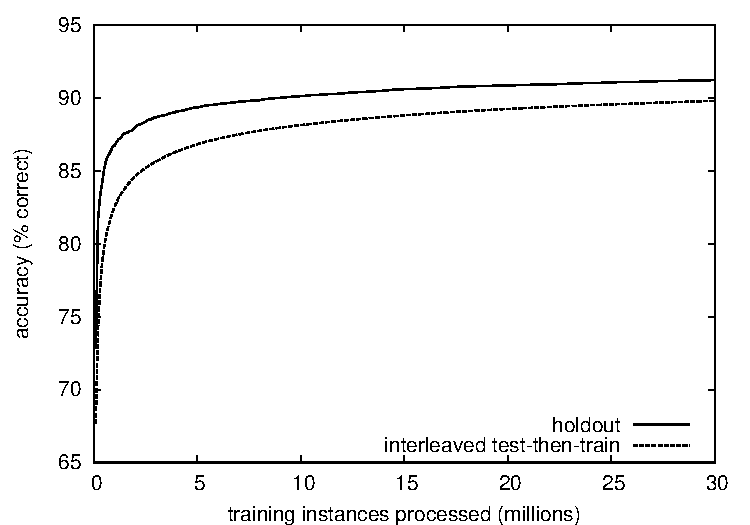
\includegraphics{figures/holdout_vs_interleaved}
\caption{Learning curves produced for the same learning situation by two different evaluation methods, recorded every 100,000 examples.}
\label{fig:holdout_vs_interleaved}
\end{figure}

Figure~\ref{fig:holdout_vs_interleaved} is an example of how learning curves can differ between the two approaches given an identical learning algorithm and data source. The holdout method measures immediate accuracy at a particular point, without memory of previous performance. During the first few million training examples the graph is not smooth. If the test set were small thus unreliable or the algorithm more unstable then fluctuations in accuracy could be much more noticeable. The interleaved method by contrast measures the average accuracy achieved to a given point, thus after 30 million training examples, the generalization accuracy has been measured on every one of the 30 million examples, rather than the independent one million examples used by the holdout. This explains why the interleaved curve is smooth. It also explains why the estimate of accuracy is more pessimistic, because during early stages of learning the model was less accurate, pulling the average accuracy down.

The interleaved method makes measuring estimates of both time and accuracy more difficult. It could be improved perhaps using a modification that introduces exponential decay, but this possibility is reserved for future work. The holdout evaluation method offers the best of both schemes, as the averaged accuracy that would be obtained via interleaved test-then-train can be estimated by averaging consecutive ranges of samples together. Having considered the relative merits of the approaches, the holdout method constitutes the foundation of the experimental framework described next.

\section{Testing Framework}
\label{sec:framework}

\begin{algorithm}
\caption{Evaluation procedure.}
\begin{algorithmic}
\STATE Fix $m_{bound}$, the maximum amount of memory allowed for the model
\STATE Hold out $n_{test}$ examples for testing
\WHILE{further evaluation is desired}
\STATE start training timer
\FOR{$i=1$ to $n_{train}$}
\STATE get next example $e_{train}$ from training stream
\STATE train and update model with $e_{train}$, ensuring that $m_{bound}$ is obeyed
\ENDFOR
\STATE stop training timer and record training time
\STATE start test timer
\FOR{$i=1$ to $n_{test}$}
\STATE get next example $e_{test}$ from test stream
\STATE test model on $e_{test}$ and update accuracy
\ENDFOR
\STATE stop test timer and record test time
\STATE record model statistics (accuracy, size etc.)
\ENDWHILE
\end{algorithmic}
\label{alg:eval}
\end{algorithm}

Algorithm~\ref{alg:eval} lists pseudo-code of the evaluation procedure used for experimental work in this \thesisc. The process is similar to that used by Domingos and Hulten~\cite{vfdt}, the study that was found to have the most thorough evaluation practices of those surveyed in Section~\ref{sec:dsevalsurvey}. It offers flexibility regarding which statistics are captured, with the potential to track many behaviours of interest.

The $n_{train}$ parameter determines how many examples will be used for training before an evaluation is performed on the test set. A set of $n_{test}$ examples is held aside for testing. In the data stream case without concept drift this set can be easily populated by collecting the first $n_{test}$ examples from the stream.

To get reliable timing estimates, $n_{train}$ and $n_{test}$ need to be sufficiently large. In the actual implementation, the timer measured the CPU runtime of the relevant thread, in an effort to reduce problems caused by the multithreaded operating system sharing other tasks. In all experiments, $n_{test}$ was set to one million examples, which helps to measure timing but also ensures reliability of the accuracy estimates, where according to Table~\ref{tab:evalsurvey1} previous studies in the field have typically used a tenth of this amount or even less.

The framework is designed to test an algorithm that tends to accumulate information over time, so the algorithm will desire more memory as it trains on more examples. The algorithm needs to be able to limit the total amount of memory used, thus obey $m_{bound}$, no matter how much training takes place.

\begin{figure}
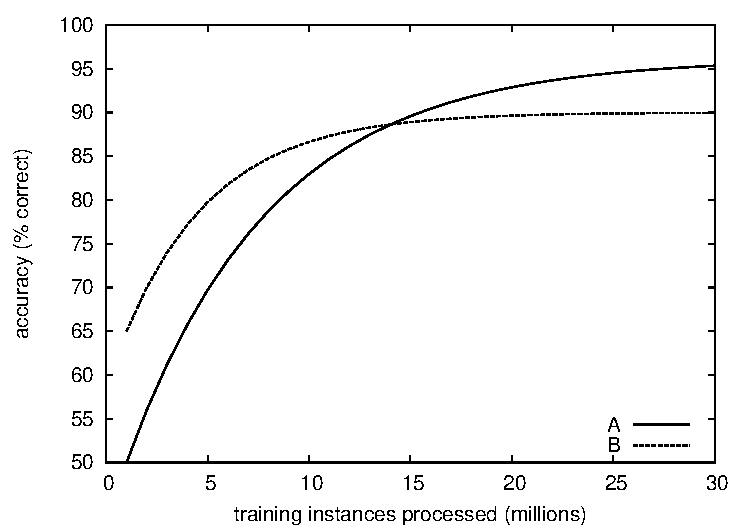
\includegraphics{figures/AvsB}
\caption{Learning curves demonstrating the problem of stopping early.}
\label{fig:learningcurves}
\end{figure}

One of the biggest issues with the evaluation is deciding when to stop training and start testing. In small memory situations, some algorithms will reach a point where they have exhausted all memory and can no longer learn new information. At this point the experiment can be terminated, as the results will not change from that point.

More problematic is the situation where time or training examples are exhausted before the final level of performance can be observed.
Consider Figure~\ref{fig:learningcurves}. Prior to 14 million examples, algorithm B is the clear choice in terms of accuracy, however in the long run it does not reach the same level of accuracy as algorithm A. Which algorithm is actually better depends on the application. If there is a shortage of time or data, algorithm B may be the better choice. Not only this, but if the models are employed for prediction during early stages of learning, then algorithm B will be more useful at the beginning.

To rule out any effect that data order may have on the learning process, the evaluation procedure may be run multiple times, each time with a different set of training data from the same problem. The observations gathered from each run can then be averaged into a single result. An advantage of this approach is that the variance of behaviour can also be observed. Ideally the data between runs will be unique, as is possible with synthetically generated or other abundant data sources. If data is lacking at least the training examples can be reordered.

An ideal method of evaluation would wait until an accuracy plateau is observable for every candidate before termination. It would also run multiple times with different data orders to establish confidence in the results. Unfortunately neither of these scenarios are feasible considering the large amount of experimental work needed. % for this \thesisc.

\BEGINOMIT
To see why this is so, consider the time required to run all of the experiments in this \thesisc. There are 19 different data sources. There are three memory limits, but only two are counted here because experiments terminate early in the smallest environment. There are at least 20 different variants of algorithm being tested, which underestimates the full amount of work by ignoring background experimentation such as performing bias/variance decomposition in Chapter~\ref{chap:improvecompare}.
If ten hours are required per run, the total time required is:
\begin{center}
19 data sets $\times$ 2 environments $\times$ 20 algorithms $\times$ 10 hours = 7600 hours
\end{center}
So a conservative estimate is that 317 days or more than 45 weeks of linear computing time is required to generate the results. Running the evaluation process in parallel is straightforward, so with several machines the practical runtime can be reduced, but not without access to substantial computing resources. Requiring multiple runs or more than ten hours per run will readily inflate the computing time needed.

For this practical reason, all experiments allowed a maximum of ten hours training time. The time required for the entire evaluation process is slightly longer than ten hours due to time required for testing, which is not included in the limit. Aside from algorithms being tested in the smallest memory environment, nearly every algorithm trained for the full ten hour period and could have continued for longer if permitted. The only exceptions were a small number of cases where the most memory-hungry ensemble methods described in Chapter~\ref{chap:improvecompare} became incapable of doing any more work in the memory allowed.

Regarding the problem that terminating evaluation too early can bias results, there are two causes of early termination, shortage of data or shortage of time. Data shortage is avoided by using synthetic data generators thereby having unlimited data. Time shortage is more problematic but as explained it is unreasonable to expect more than ten hours of training per evaluation run, which is considered to be a reasonable amount of time.
\ENDOMIT

The question of when an algorithm is superior to another is decided by looking at the final result recorded after the ten hour evaluation completed. The accuracy results are reported as percentages to two decimal places, and if a method's final accuracy reading in this context is greater than another then it is claimed to be superior. As with other similar studies there is no attempt to strictly analyze the confidence of results, although differences of several percentages are more convincing than fractional differences.

Measuring the standard error of results via multiple runs would enable the confidence of results to be more formally analyzed, but every additional run would multiply time requirements. A less expensive but useful alternative might be to examine differences between algorithms in another way, using McNemar's test~\cite{mcnemar} for example, which can be computed by tracking the agreement between competing methods on each test example. Extra analysis such as this was not considered necessary for this \thesisc, but the idea presents opportunity for future research into evaluation of data stream classification.

\BEGINOMIT
Two factors add informal confidence in the results obtained. Firstly, the class of base algorithm being studied (fully described in Chapter~\ref{chap:hoeffdingtrees}) has low sensitivity to data order, as reported previously~\cite{stresstest,ufft} and confirmed in smaller scale initial experiments. This suggests that even if multiple runs were performed and averaged, the final results would not change very much. Secondly, this study uses test set sizes that are several times larger than the largest used in previous studies, further decreasing the likelihood that methods can achieve high accuracy via chance alone.

The methodology employed is largely consistent with other studies, only on a greater scale. Where previous studies rarely trained on more than several million examples, the ten hour evaluation runs commonly involve several {\em hundreds} of millions of examples. There are two main ways that results are presented, as graphical plots and in tables. Graphical plots are interspersed with the text where they seem appropriate for demonstrating relevant behaviour. Unfortunately, because the graphs need to be of sufficient size to reasonably compare multiple methods, only selected graphs are shown. The space required to print readable graphs of every method on every data source in every environment and every interesting dimension is simply too high to justify.

\begin{figure}
\centering
\begin{tabular}{c@{}c}
\includegraphics[width=0.5\textwidth]{figures/rtcn-r1-400MB_leafacc_vs_examples} &
\includegraphics[width=0.5\textwidth]{figures/rtcn-r1-400MB_leafacc} \\
\end{tabular}
\caption{Example difference between learning curves based on training examples (left) versus training time (right).}
\label{fig:examples_vs_time}
\end{figure}

The information collected during a run of the evaluation procedure can be plotted in several ways to give a visual analysis of an algorithm's behaviour. Of critical interest is the learning curve, as discussed previously, where the accuracy of the algorithm's predictions is plotted against either time or number of training examples.
Previous studies have always plotted learning curves on a per-example basis, rather than a per-time basis that is dependent on the speed of computing hardware. This \thesis uses both styles interchangeably, which can slightly alter the appearance of relationships between methods, see Figure~\ref{fig:examples_vs_time}. The main difference between these styles is that time-based plots have every line spanning almost the full width of the graph rather than having slower methods terminating earlier. Plotted this way, per-example performance is still observable because each sample point represents a fixed number of training examples, such that more frequent points in a line represent more training examples being processed. Often with these graphs the sampling period is purposely adjusted to ensure a reasonable separation between sample points, enhancing readability. Where appropriate the sampling period is noted in the title of the graph. The difference between per-example and per-time plots can be dramatic when the speeds of algorithms differ greatly, such as the example in Figure~\ref{fig:rrbfc_gp} on page~\pageref{fig:rrbfc_gp}.

The graphs are supplemented by tables in Appendix~\ref{chap:detailedResultTables}. The tables cannot convey subtle changes over time like graphs can, but they can report the complete set of end results, allowing comparison of the key results for every method/data source/environment combination. The tables record the final readings at the end of evaluation, which is sufficient information for determining the best methods. Presented in this form the final results are meaningfully summarized in a reasonable amount of space.

The other important property of a learning algorithm besides accuracy is speed. It is important to differentiate learning speed from processing speed. Learning speed refers to the number of examples required to reach a given accuracy level. Processing speed is the rate at which examples are processed, consisting of both training and testing speeds, and can be measured in terms of examples processed per second.
When comparing algorithms, it is the relative time taken on identical hardware that is important, as the absolute times will vary depending on the power of the computing hardware.

The hardware/software environment has a large influence on the results obtained, because a ten hour time limit is completely arbitrary when computing resources are unspecified. The experimental environment was purposely kept consistent for all time-dependent experiments, as follows:
\begin{description}
\item[Hardware:] Intel Core2 6300 CPU running at 1.86Ghz with a 2048KB cache and 1GB of RAM
\item[Software:] Sun Java HotSpot Server VM (build 1.6.0\_01-b06), running under GNU/Linux Fedora core 6
\end{description}
\ENDOMIT

\section{Environments}
\label{sec:environments}

This section defines three environments that may be simulated using memory limits, since memory limits cannot be ignored and can significantly limit capacity to learn from data streams.
Potential practical deployment of data stream classification has been divided into scenarios of increasing memory utilization, from the restrictive {\em sensor} environment, to a typical consumer grade {\em handheld} PDA environment, to the least restrictive environment of a dedicated {\em server}.

Although technology advancements will mean that these environments are something of a moving target, the insights gained about the scalability of algorithms will still be valid. The environments chosen range from restrictive to generous, with an order of magnitude difference between them.

Note that when referring to memory sizes, the traditional meaning of the terms {\em kilobyte} and {\em megabyte} is adopted, such that 1 kilobyte = 1,024 bytes, and 1 megabyte = $1024^2$ bytes = 1,048,576 bytes.

\subsection{Sensor Network}
\label{sec:sensor}

This environment represents the most restrictive case, learning in 100 kilobytes of memory. Because this limit is so restrictive, it is an interesting test case for algorithm efficiency.

Sensor networks~\cite{sensornetworks, sensornetworksbook} are a hot topic of research, and typically the nodes designed for these networks are low power devices with limited resources. In this setting it is often impractical to dedicate more than hundreds of kilobytes to processes because typically such devices do not support much working memory.

When memory limits are in the order of kilobytes, other applications requiring low memory usage also exist, such as specialized hardware in which memory is expensive. An example of such an application is CPU branch prediction, as explored by Fern and Givan~\cite{branchpred}. Another example is a small `packet sniffer' device designed to do real-time monitoring of network traffic~\cite{packetsniff}.

\subsection{Handheld Computer}
\label{sec:handheld}

In this case the algorithm is allowed 32 megabytes of memory. This simulates the capacity of lightweight consumer devices designed to be carried around by users and fit into a shirt pocket.

The ability to do analysis {\em on site} with a handheld device is desirable for certain applications. The papers~\cite{vehicle} and~\cite{stockmarket} describe systems for analysing vehicle performance and stockmarket activity respectively. In both cases the authors describe the target computing hardware as personal handheld devices with 32 megabytes. Horovitz et al.~\cite{gaberroadsafety} describe a road safety application using a device with 64 megabytes.

The promise of ubiquitous computing is getting closer with the widespread use of mobile phones, which with each generation are evolving into increasingly more powerful and multifunctional devices. These too fall into this category, representing large potential for portable machine learning given suitable algorithms. Imielinski and Nath~\cite{wirelessgraffiti} present a vision of this future `dataspace'.

\subsection{Server}
\label{sec:server}

This environment simulates either a modern laptop/desktop computer or server dedicated to processing a data stream. The memory limit assigned in this environment is 400 megabytes. Although at the time of writing this \thesis a typical desktop computer may have several gigabytes of RAM, it is still generous to set aside this much memory for a single process. Considering that several algorithms have difficulty in fully utilizing this much working space, it seems sufficiently realistic to impose this limit.

A practical reason for imposing this limit is that the experiments need to terminate in reasonable time. In cases where memory is not filled by an algorithm it is harder to judge what the behaviour will be in the theoretical limit, but the practical ten hour limit is an attempt to run for sufficient time to allow accuracy to plateau.

There are many applications that fit into this higher end of the computing scale. An obvious task is analysing data arising from the Internet, as either web searches~\cite{webmine}, web usage~\cite{webusage}, site logs~\cite{weblogs} or click streams~\cite{clickstreams}. Smaller scale computer networks also produce traffic of interest~\cite{minenetwork}, as do other telecommunication activities~\cite{telecommunications}, phone call logs for example. Banks may be interested in patterns of ATM transactions~\cite{minebank}, and retail chains and online stores will want details about customer purchases~\cite{ecommerceapp}. Further still, there is the field of scientific observation~\cite{minescientific}, which can be astronomical~\cite{astronomical}, geophysical~\cite{geophysical}, or the massive volume of data output by particle accelerator experiments~\cite{particleaccelerator}. All of these activities are sources of data streams that users will conceivably want to analyze in a server environment.

\section{Data Sources}
\label{sec:datasets}

For the purposes of research into data stream classification there is a shortage of suitable and publicly available real-world benchmark data sets. The UCI ML~\cite{uci} and KDD~\cite{ucikdd} archives house the most common benchmarks for machine learning algorithms, but many of those data sets are not suitable for evaluating data stream classification. The KDD archive has several large data sets, but not classification problems with sufficient examples. The {\em Forest Covertype} data set is one of the largest, and that has less than 600,000 examples.

To demonstrate their systems, several researchers have used private real-world data that cannot be reproduced by others. Examples of this include the web trace from the University of Washington used by Domingos and Hulten to evaluate VFDT~\cite{vfdt}, and the credit card fraud data used by Wang et al.~\cite{cdensemble} and Chu and Zaniolo~\cite{fastlightboost}.

More typically, researchers publish results based on synthetically generated data.
In many of these cases, the authors have invented unique data generation schemes for the purpose of evaluating their algorithm.
Examples include the random tree generator also used to evaluate VFDT, and the custom generators described in Oza and Russell~\cite{ozaexp}, Street and Kim~\cite{sea} and Chu and Zaniolo~\cite{fastlightboost}.
Synthetic data has several advantages---it is easier to reproduce and there is little cost in terms of storage and transmission.
Despite these advantages there is a lack of established and widely used synthetic data streams. 

\begin{table}
\caption{Properties of the data sources.}
\centering
\begin{tabular}{|l|c|c|c|}
\hline
name     &    nominal    &    numeric    &    classes    \\
\hline
{\sc rts/rtsn}    &    10    &    10    &    2    \\
{\sc rtc/rtcn}    &    50    &    50    &    2    \\
{\sc rrbfs}    &    0    &    10    &    2    \\
{\sc rrbfc}    &    0    &    50    &    2    \\
{\sc led}    &    24    &    0    &    10    \\
{\sc wave21}    &    0    &    21    &    3    \\
{\sc wave40}    &    0    &    40    &    3    \\
{\sc genF1-F10}    &    6    &    3    &    2    \\
\hline
\end{tabular}
\label{tab:datasets}
\end{table}

For this \thesisc, the data generators most commonly found in the literature have been collected, and and an extra scheme (RBF) has been introduced. For ease of reference, each data set variation is assigned a short name. The basic properties of each are summarized in Table~\ref{tab:datasets}.

\BEGINOMIT
\subsection{Lack of Real-World Data}
\label{sec:reallack}

The first place to find real-world benchmark data for evaluating machine learning algorithms is the UCI machine learning repository~\cite{uci}. Larger real-world data sets can be found in the UCI KDD archive~\cite{ucikdd}, which was established to serve the needs of larger scale benchmarking.

Table~\ref{tab:ucikddsizes} summarizes the sizes of the data sets in the KDD archive that were found to best suit the task of evaluating classification. The archive has other large data sets that are not considered because they are intended for topics with different requirements such as text categorization and time series classification.

The data set with the most examples is {\em KDD Cup 1999} which has nearly five million training examples. The task is to detect network intrusion attempts. After initial experiments with this data it became clear that it is not a very useful benchmark---it is too easy to achieve near-perfect accuracy, there are many classes with a highly imbalanced distribution of examples between classes, making it hard to discern anything from the accuracies measured for competing methods. Further analysis of the data revealed that there is a high number of repeated examples, such that the number of unique training examples is several times less than the total number of examples specified. Brugger~\cite{kdd99flaw} has expressed concerns that this data set is flawed.

\begin{table}
\caption{Sizes of data sets in UCI KDD archive that are suitable for evaluating classification.}
\centering
\begin{tabular}{|l|r|r|}
\hline					
name	&	attributes	&	training/test examples	\\
\hline					
Census-Income	&	40	&	199,523/99,762	\\
COIL	&	17	&	340	\\
Corel Image	&	89	&	68,040	\\
Forest Covertype	&	54	&	581,012	\\
Insurance Company (COIL2000)	&	86	&	5,822/4,000	\\
Internet Usage	&	71	&	10,108	\\
IPUMS	&	60	&	233,584	\\
KDD Cup 1998	&	481	&	95,412	\\
KDD Cup 1999	&	40	&	4,898,430/311,029	\\
MS Anonymous Web	&	294	&	32,711	\\
\hline					
\end{tabular}
\label{tab:ucikddsizes}
\end{table}

The next largest data set available is {\em Forest Covertype}, a more reasonable classification benchmark. It is not surprising that this data set has been used in several papers on data stream classification~\cite{vfdtc,ozaexp}, given the lack of alternatives.

For the style of evaluation required by this \thesisc, where several hundreds of millions of training examples are required to test genuine ability to handle data streams, these data sets are simply not adequate. The need to rely on artificial data is unfortunate but necessary.
\ENDOMIT

\subsection{Random Tree Generator}
\label{sec:randtrees}

This generator is based on that proposed by Domingos and Hulten~\cite{vfdt}, producing concepts that in theory should favour decision tree learners. It constructs a decision tree by choosing attributes at random to split, and assigning a random class label to each leaf. Once the tree is built, new examples are generated by assigning uniformly distributed random values to attributes which then determine the class label via the tree.

The generator has parameters to control the number of classes, attributes, nominal attribute labels, and the depth of the tree. For consistency between experiments, two random trees were generated and fixed as the base concepts for testing---one {\em simple} and the other {\em complex}, where complexity refers to the number of attributes involved and the size of the tree.

The simple random tree ({\sc rts}) has ten nominal attributes with five values each, ten numeric attributes, two classes, a tree depth of five, with leaves starting at level three and a 0.15 chance of leaves thereafter. The final tree has 741 nodes, 509 of which are leaves.

The complex random tree ({\sc rtc}) has 50 nominal attributes with five values each, 50 numeric attributes, two classes, a tree depth of ten, with leaves starting at level five and a 0.15 chance of leaves thereafter. The final tree has 127,837 nodes, 90,259 of which are leaves.

A degree of noise can be introduced to the examples after generation. In the case of discrete attributes and the class label, a probability of noise parameter determines the chance that any particular value is switched to something other than the original value. For numeric attributes, a degree of random noise is added to all values, drawn from a random Gaussian distribution with standard deviation equal to the standard deviation of the original values multiplied by noise probability.
The streams {\sc rtsn} and {\sc rtcn} are introduced by adding 10\% noise to the respective random tree data streams. It is hoped that experimenting with both noiseless and noisy versions of a problem can give insight into how well the algorithms manage noise.

\subsection{Random RBF Generator}
\label{sec:randrbf}

This generator was devised to offer an alternate concept type that is not necessarily as easy to capture with a decision tree model.

The RBF (Radial Basis Function) generator works as follows:
A fixed number of random centroids are generated. Each center has a random position, a single standard deviation, class label and weight. New examples are generated by selecting a center at random, taking weights into consideration so that centers with higher weight are more likely to be chosen. A random direction is chosen to offset the attribute values from the central point. The length of the displacement is randomly drawn from a Gaussian distribution with standard deviation determined by the chosen centroid. The chosen centroid also determines the class label of the example. This effectively creates a normally distributed hypersphere of examples surrounding each central point with varying densities. Only numeric attributes are generated.

{\sc rrbfs} refers to a simple random RBF data set---100 centers and ten attributes. 
{\sc rrbfc} is more complex---1000 centers and 50 attributes. 
Both are two class problems.

\subsection{LED Generator}
\label{sec:led}

This data source originates from the CART book~\cite{cart}. An implementation in C was donated to the UCI~\cite{uci} machine learning repository by David Aha. The goal is to predict the digit displayed on a seven-segment LED display, where each attribute has a 10\% chance of being inverted. It has an optimal Bayes classification rate of 74\%. The particular configuration of the generator used for experiments ({\sc led}) produces 24 binary attributes, 17 of which are irrelevant.

\subsection{Waveform Generator}
\label{sec:waveform}

This generator shares its origins with {\sc led}, and was also donated by David Aha to the UCI repository. The goal of the task is to differentiate between three different classes of waveform, each of which is generated from a combination of two or three {\em base} waves. The optimal Bayes classification rate is known to be 86\%. There are two versions of the problem. {\sc wave21} has 21 numeric attributes, all of which include noise. {\sc wave40} introduces an additional 19 irrelevant attributes.

\subsection{Function Generator}
\label{sec:genFx}

This generator was introduced by Agrawal et al. in~\cite{dbmine}, and was a common source of data for early work on scaling up decision tree learners~\cite{sliq,sprint,rainforest}.

\begin{table}
\caption{Function generator attributes.}
\centering
\begin{tabular}{|l|l|l|}
\hline
name     &    description    &    values    \\
\hline
{\it salary} & salary & uniformly distributed from 20K to 150K \\
{\it commission} & commission & {\bf if} ({\it salary} $<$ 75K) {\bf then} 0 {\bf else} \\
& & uniformly distributed from 10K to 75K \\
{\it age} & age & uniformly distributed from 20 to 80 \\
{\it elevel} & education level & uniformly chosen from 0 to 4 \\
{\it car} & make of car & uniformly chosen from 1 to 20 \\
{\it zipcode} & zip code of town & uniformly chosen from 9 zipcodes \\
{\it hvalue} & value of house & uniformly distributed \\
& & from 0.5$k$100000 to 1.5$k$100000  \\
& & where $k \in \{1...9\}$ depending on {\it zipcode} \\
{\it hyears} & years house owned & uniformly distributed from 1 to 30  \\
{\it loan} & total loan amount & uniformly distributed from 0 to 500K  \\
\hline
\end{tabular}
\label{tab:agrawalAtts}
\end{table}

The generator produces a stream containing nine attributes, six numeric and three categorical, described in Table~\ref{tab:agrawalAtts}. Although not explicitly stated by the authors, a sensible conclusion is that these attributes describe hypothetical loan applications.

There are ten functions defined for generating binary class labels from the attributes. The functions are listed in Figures~\ref{fig:agrawalFuncs1} and~\ref{fig:agrawalFuncs2}. Presumably these determine whether the loan should be approved. For the experiments the ten functions are used as described, with a perturbation factor of 5\% (referred to as {\sc genF1}-{\sc genF10}). 
Perturbation shifts numeric attributes from their true value, adding an offset drawn randomly from a uniform distribution, the range of which is a specified percentage of the total value range.

\begin{figure}
\begin{enumerate}
\item
{\bf if} ({\it age} $< 40$) $\lor$ ({\it age} $\ge 60$) {\bf then}\\
\hspace*{1em} {\it group} = A\\
{\bf else}\\
\hspace*{1em} {\it group} = B\\
\item
{\bf if} (({\it age} $< 40$) $\land$ ($50000 \le$ {\it salary} $\le 100000$)) $\lor$\\
\hspace*{1em} (($40 \le$ {\it age} $< 60$) $\land$ ($75000 \le$ {\it salary} $\le 125000$)) $\lor$\\
\hspace*{1em} (({\it age} $\ge 60$) $\land$ ($25000 \le$ {\it salary} $\le 75000$)) {\bf then}\\
\hspace*{1em} {\it group} = A\\
{\bf else}\\
\hspace*{1em} {\it group} = B\\
\item
{\bf if} (({\it age} $< 40$) $\land$ ({\it elevel} $\in [0..1$])) $\lor$\\
\hspace*{1em} (($40 \le$ {\it age} $< 60$) $\land$ ({\it elevel} $\in [1..3]$)) $\lor$\\
\hspace*{1em} (({\it age} $\ge 60$) $\land$ ({\it elevel} $\in [2..4]$)) {\bf then}\\
\hspace*{1em} {\it group} = A\\
{\bf else}\\
\hspace*{1em} {\it group} = B \\
\item
{\bf if} (({\it age} $< 40$) $\land$ ({\it elevel} $\in [0..1]$ ?\\
\hspace*{2em} ($25000 \le$ {\it salary} $\le 75000$) : ($50000 \le$ {\it salary} $\le 100000$))) $\lor$\\
\hspace*{1em} (($40 \le$ {\it age} $< 60$) $\land$ ({\it elevel} $\in [1..3]$ ?\\
\hspace*{2em} ($50000 \le$ {\it salary} $\le 100000$) : ($75000 \le$ {\it salary} $\le 125000$))) $\lor$\\
\hspace*{1em} (({\it age} $\ge 60$) $\land$ ({\it elevel} $\in [2..4]$ ?\\
\hspace*{2em} ($50000 \le$ {\it salary} $\le 100000$) : ($25000 \le$ {\it salary} $\le 75000$))) {\bf then}\\
\hspace*{1em} {\it group} = A\\
{\bf else}\\
\hspace*{1em} {\it group} = B\\
\item
{\bf if} (({\it age} $< 40$) $\land$ (($50000 \le$ {\it salary} $\le 100000$) ?\\
\hspace*{2em} ($100000 \le$ {\it loan} $\le 300000$) : ($200000 \le$ {\it loan} $\le 400000$))) $\lor$\\
\hspace*{1em} (($40 \le$ {\it age} $< 60$) $\land$ (($75000 \le$ {\it salary} $\le 125000$) ?\\
\hspace*{2em} ($200000 \le$ {\it loan} $\le 400000$) : ($300000 \le$ {\it loan} $\le 500000$))) $\lor$\\
\hspace*{1em} (({\it age} $\ge 60$) $\land$ (($25000 \le$ {\it salary} $\le 75000$) ?\\
\hspace*{2em} ($30000 \le$ {\it loan} $\le 500000$) : ($100000 \le$ {\it loan} $\le 300000$))) {\bf then}\\
\hspace*{1em} group = A\\
{\bf else}\\
\hspace*{1em} group = B\\
\end{enumerate}
\caption{Generator functions 1-5.}
\label{fig:agrawalFuncs1}
\end{figure}

\begin{figure}
\begin{enumerate}
\setcounter{enumi}{5}
\item
{\bf if} (({\it age} $< 40$) $\land$ ($50000 \le$ ({\it salary} + {\it commission}) $\le 100000$)) $\lor$\\
\hspace*{1em} (($40 \le$ {\it age} $< 60$) $\land$ ($75000 \le$ ({\it salary} + {\it commission}) $\le 125000$)) $\lor$\\
\hspace*{1em} (({\it age} $\ge 60$) $\land$ ($25000 \le$ ({\it salary} + {\it commission}) $\le 75000$)) {\bf then}\\
\hspace*{1em} {\it group} = A\\
{\bf else}\\
\hspace*{1em} {\it group} = B\\
\item
{\bf if} (0.67 $\times$ ({\it salary} + {\it commission}) $-$ 0.2 $\times$ {\it loan} $-$ 20000 $> 0$) {\bf then}\\
\hspace*{1em} {\it group} = A\\
{\bf else}\\
\hspace*{1em} {\it group} = B\\
\item
{\bf if} (0.67 $\times$ ({\it salary} + {\it commission}) $-$ 5000 $\times$ {\it elevel} $-$ 20000 $> 0$) {\bf then}\\
\hspace*{1em} {\it group} = A\\
{\bf else}\\
\hspace*{1em} {\it group} = B\\
\item
{\bf if} (0.67 $\times$ ({\it salary} + {\it commission}) $-$ 5000 $\times$ {\it elevel}\\
\hspace*{1em} $-$ 0.2 $\times$ {\it loan} $-$ 10000 $> 0$) {\bf then}\\
\hspace*{1em} {\it group} = A\\
{\bf else}\\
\hspace*{1em} {\it group} = B\\
\item
{\bf if} ({\it hyears} $\ge 20$) {\bf then}\\
\hspace*{1em} {\it equity} = 0.1 $\times$ {\it hvalue} $\times$ ({\it hyears} $-$ 20)\\
{\bf else}\\
\hspace*{1em} {\it equity} = 0\\
\\
{\bf if} (0.67 $\times$ ({\it salary} + {\it commission}) $-$ 5000 $\times$ {\it elevel}\\
\hspace*{1em} $-$ 0.2 $\times$ {\it equity} $-$ 10000 $> 0$) {\bf then}\\
\hspace*{1em} {\it group} = A\\
{\bf else}\\
\hspace*{1em} {\it group} = B\\
\end{enumerate}
\caption{Generator functions 6-10.}
\label{fig:agrawalFuncs2}
\end{figure}

\section{Generation Speed and Data Size}
\label{sec:genspeed}

During evaluation the data is generated on-the-fly. This directly influences the amount of training examples that can be supplied in any given time period.

\begin{table}
\caption{Generation speed and data size of the streams.}
\centering
\begin{tabular}{|r|r|r|r|r|r|}
\hline		
	&	examples	&		&		&	examples in	&		\\
	&	per second	&		&	bytes per	&	10 hours	&	terabytes in	\\
stream	&	(thousands)	&	attributes	&	example	&	(millions)	&	10 hours	\\
\hline											
{\sc rts}	&	274	&	20	&	168	&	9866	&	1.50	\\
{\sc rtsn}	&	97	&	20	&	168	&	3509	&	0.53	\\
{\sc rtc	}&	19	&	100	&	808	&	667	&	0.49	\\
{\sc rtcn}	&	9	&	100	&	808	&	338	&	0.25	\\
{\sc rrbfs}	&	484	&	10	&	88	&	17417	&	1.39	\\
{\sc rrbfc}	&	120	&	50	&	408	&	4309	&	1.60	\\
{\sc led	}&	260	&	24	&	200	&	9377	&	1.71	\\
{\sc wave21}	&	116	&	21	&	176	&	4187	&	0.67	\\
{\sc wave40}	&	56	&	40	&	328	&	2003	&	0.60	\\
{\sc genF1}	&	527	&	9	&	80	&	18957	&	1.38	\\
{\sc genF2}	&	531	&	9	&	80	&	19108	&	1.39	\\
{\sc genF3}	&	525	&	9	&	80	&	18917	&	1.38	\\
{\sc genF4}	&	523	&	9	&	80	&	18838	&	1.37	\\
{\sc genF5}	&	518	&	9	&	80	&	18653	&	1.36	\\
{\sc genF6}	&	524	&	9	&	80	&	18858	&	1.37	\\
{\sc genF7}	&	527	&	9	&	80	&	18977	&	1.38	\\
{\sc genF8}	&	524	&	9	&	80	&	18848	&	1.37	\\
{\sc genF9}	&	519	&	9	&	80	&	18701	&	1.36	\\
{\sc genF10}	&	527	&	9	&	80	&	18957	&	1.47	\\
\hline											
\end{tabular}
\label{tab:dsspeeds}
\end{table}


The speed of the MOA data generators was measured in the experimental hardware/software environment. The results are shown in Table~\ref{tab:dsspeeds}, where the full speed possible for generating each stream was estimated by timing how long it took to generate ten million examples. The possible speed ranges from around nine thousand examples per second on {\sc rtcn} to over 500 thousand examples per second for the function generators {\sc genF$x$}. The biggest factor influencing speed is the number of attributes being generated, hence the fastest streams are those with the least attributes. The addition of noise to the streams also has a major impact on the speeds---going from {\sc rts} to {\sc rtsn} and from {\sc rtc} to {\sc rtcn} causes the speed to roughly halve, where the only difference between these variants is the addition of noise. 
This result is consistent with the notion that a dominant cost of generating the streams is the time needed to generate random numbers, as adding noise involves producing at least one additional random number per attribute.

In terms of the sizes of the examples, the assumption is made that storage of each attribute and class label requires eight bytes of memory, matching the actual Java implementation where all values are stored as double precision floating point numbers (Section~\ref{sec:javaimpl}). Certain attribute types could be stored more efficiently, but this approach offers maximum flexibility, and storing continuous values in less space would reduce precision.

For example, considering an evaluation period of ten hours, the total number of examples that can be produced at full speed range from around 300 to 19,000 million. With the eight-byte-per-attribute assumption, this translates to between approximately 0.25 to 1.7 terabytes of data. With data volumes of this magnitude the choice of generating data on-the-fly is justified, a solution that is cheaper than finding resources to store and retrieve several terabytes of data.

\BEGINOMIT
\section{Summary}

Aiming to best meet user requirements for data stream classification, the necessity for memory-limited algorithms has been argued. Looking first at prior studies, a comprehensive evaluation framework has been described, testing methods on a scale not previously attempted. The framework is complemented with three simulated memory-limited environments, defined to cover the range of potential deployment scenarios.  A suite of synthetic benchmark data streams have been proposed, and their properties studied. The evaluation framework enables experimental work and comparison of algorithms to be performed throughout the thesis.
\ENDOMIT